\begin{filecontents*}{references.bib}
@book{goodfellow2016deep,
  title={Deep Learning},
  author={Goodfellow, Ian and Bengio, Yoshua and Courville, Aaron},
  year={2016},
  publisher={MIT Press}
}
\end{filecontents*}

\documentclass{article} % For LaTeX2e
\usepackage{iclr2025,times}

% Optional math commands from https://github.com/goodfeli/dlbook_notation.
\input{math_commands.tex}

\usepackage{hyperref}
\usepackage{url}
\usepackage{graphicx}
\usepackage{booktabs}
\usepackage{amsmath}
\usepackage{amssymb}
\usepackage{mathtools}
\usepackage[capitalize,noabbrev]{cleveref}

\graphicspath{{../figures/}} % To reference your generated figures, name the PNGs directly. DO NOT CHANGE THIS.

\title{
Conflict-Memory Feedback for Decoupled Multi-Agent Scheduling:\\
Helpful in Bottlenecks, Fragile Elsewhere
}

\author{Anonymous}

%\iclrfinalcopy % Uncomment for camera-ready version, but NOT for submission.
\begin{document}

\maketitle

\begin{abstract}
Decoupled multi-agent scheduling is attractive because task assignment can be solved cheaply before path planning, but this modularity ignores downstream congestion. We study whether a lightweight ``conflict memory'' can feed congestion information back into assignment without full joint optimization. Our intended idea was to learn from MAPF conflict logs, but the current prototype only realizes a weaker proxy: a CNN predicts short-horizon congestion maps from agent and task occupancy, and the predicted path congestion is added to a greedy assignment cost. In three synthetic warehouse layouts, this proxy sometimes helps. The best setting, selected by end-task utility rather than predictor loss, improves mean throughput by about 7.1\% over a standard decoupled baseline. However, the gains are highly uneven: improvements are concentrated in bottlenecked and dense-obstacle layouts at medium load, while sparse layouts remain near zero and several low-load settings become worse than the baseline. A particularly important pitfall is that the lowest validation loss occurs at 60 epochs, whereas the best scheduling performance occurs at 30 epochs. Our conclusion is therefore mixed: reusable congestion structure does exist, but learning a good congestion predictor is easier than turning it into a robust allocation signal.
\end{abstract}

\section{Introduction}
\label{sec:intro}

A standard way to scale multi-agent scheduling is to decouple task allocation from path planning. The allocator first matches agents to tasks, and a motion planner resolves the resulting traffic afterward. This is computationally convenient, but it also creates a familiar failure mode: assignments that look cheap under distance can send many agents through the same corridor, doorway, or obstacle gap.

The motivating hypothesis behind Conflict Memory Allocation (CMA) is simple. Path-planning conflicts are not purely random; they reflect recurring interactions between task geography and environment topology. If those recurring patterns can be summarized as a reusable memory map, then the allocator could penalize assignments that are likely to recreate the same congestion. In principle, this should recover part of the benefit of tighter coupling while preserving the simplicity of a decoupled pipeline.

This paper reports a smaller and less clean result than that original vision. Our available prototype does \emph{not} yet consume explicit CBS-style conflict logs, and it does not compare against a fully coupled MAPF solver. Instead, it learns a congestion proxy from occupancy grids and injects that prediction into a decoupled greedy assignment rule. Even under this simplified setup, the idea is only partially successful: we observe clear gains in harder layouts, but the method is unstable across training length, environment, and agent count.

That mismatch is the main contribution. We show that utility and predictor quality can disagree: the model with the lowest validation loss is not the model that yields the best scheduling performance. The feedback signal is useful mainly in structured, high-pressure layouts; in easy layouts, or at the wrong load, it can be neutral or harmful. This makes CMA a good fit for the ICBINB setting: the intuition is plausible, but a weak conflict proxy is not enough to make the feedback loop reliable.

\section{Related Work}
\label{sec:related}

Our predictor is a plain CNN rather than a new architecture, and its learning setup follows standard supervised dense prediction from structured spatial inputs \citep{goodfellow2016deep}. The point of the paper is therefore not representation novelty, but a downstream pitfall: a model that looks better under its surrogate loss may still be a worse decision signal once embedded in a control loop. That gap between training objective and deployment objective is a recurring concern in deep learning systems \citep{goodfellow2016deep}.

\section{Background}
\label{sec:background}

Let agent $i$ at position $s_i$ be assigned to task $j$ at position $g_j$. A purely decoupled allocator uses a distance-like cost $d_{ij}$ and ignores the traffic pattern induced by all other assignments. CMA adds a soft memory penalty over an estimated path $\hat{\pi}_{ij}$:
\begin{equation}
c_{ij} = d_{ij} + \lambda \sum_{x \in \hat{\pi}_{ij}} \hat{M}(x),
\label{eq:cma-cost}
\end{equation}
where $\hat{M}$ is a learned congestion map and $\lambda$ is a tunable weight. If $\hat{M}$ correctly highlights cells that repeatedly become crowded, then the allocator can avoid sending many agents through the same region at the same time. In the ideal version of the idea, $\hat{M}$ would be derived from actual path-planning conflicts; in the present study, it is derived from a weaker proxy: predicted short-horizon occupancy congestion.

\section{Method}
\label{sec:method}

Our prototype uses a two-channel grid input containing agent occupancy and active-task occupancy. A three-layer CNN predicts a single congestion channel over the map. The training target is the simulator's normalized short-horizon congestion estimate: given provisional assignments, each agent contributes discounted occupancy mass along its next few path steps, so near-term overlap creates a brighter target map.

At decision time, we compare two methods. \textbf{Standard decoupled} assigns tasks greedily using only Manhattan distance. \textbf{Conflict memory allocation} uses the same greedy matcher but replaces the distance-only cost with \cref{eq:cma-cost}, where the path penalty is the sum of predicted congestion along a simple obstacle-aware path estimate. In other words, the only behavioral difference between the two methods is whether the learned memory map perturbs the assignment cost.

This implementation is intentionally a proxy. It has no explicit vertex or edge conflicts, no historical decay mechanism, and no graph neural component. The paper's claim is therefore narrow: even a weak conflict-memory surrogate can reveal both the promise and the brittleness of congestion feedback.

\section{Experimental Setup}
\label{sec:experimental_setup}

We evaluate on three $20 \times 20$ warehouse layouts generated by the provided simulator: a sparse warehouse, a bottleneck warehouse with a central cross-shaped choke point, and a dense-obstacle warehouse. Each episode has 30 active tasks and either 20, 30, 40, or 50 agents, and lasts 100 simulator steps. Throughput is reported as completed tasks per minute. Congestion is reported as the cumulative number of cells containing more than two agents at a step; this is an occupancy-based proxy, not a MAPF collision count.

Training uses 800 synthetic states: 300 sparse, 300 bottleneck, and 200 dense-obstacle samples. Validation uses 100 held-out dense-obstacle samples only. We train the predictor for 30, 60, 90, or 120 epochs with Adam, learning rate $10^{-3}$, batch size 32, and MSE loss. Every evaluation point averages 5 episodes, and plotted error bars are intended only as qualitative variation indicators rather than as a substitute for formal significance tests.

Two caveats are important. First, the validation distribution is narrower than the deployment distribution, so a low validation loss need not imply good average scheduling utility. Second, because no MAPF solver is used, the study should be interpreted as a congestion-proxy pilot rather than a full test of conflict-memory learning.

\begin{figure}[t]
\centering
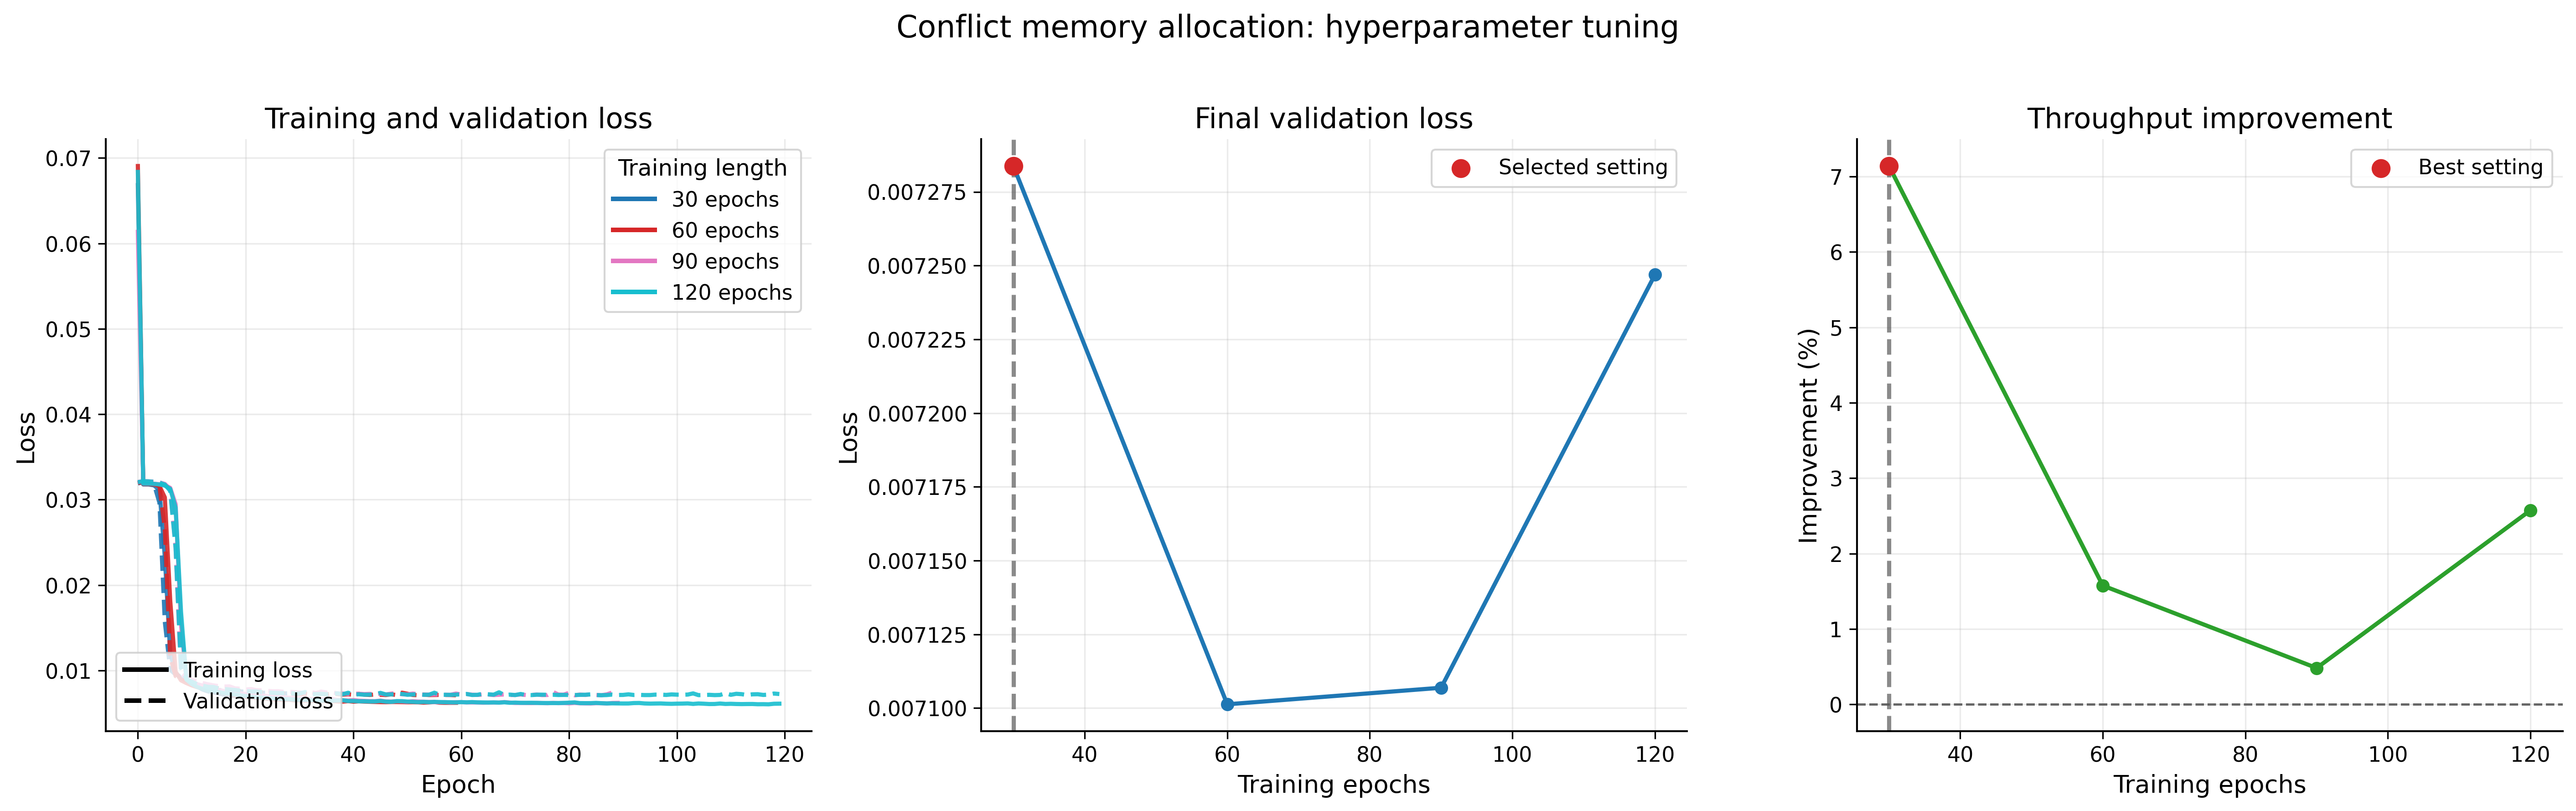
\includegraphics[width=\textwidth]{figure_1_hyperparameter_tuning.png}
\caption{Hyperparameter tuning for the congestion predictor. Training and validation loss quickly flatten, and the lowest validation loss occurs at 60 epochs. The highlighted 30-epoch checkpoint is selected by downstream utility, not by validation loss: it yields about 7.1\% mean throughput improvement versus only about 1.6\% at 60 epochs. Predictor quality and scheduler utility are therefore misaligned.}
\label{fig:hyper}
\end{figure}

\section{Experiments}
\label{sec:experiments}

\paragraph{Hyperparameter selection is not utility aligned.}
\Cref{fig:hyper} is the clearest negative result. The predictor trains smoothly: the loss curves fall quickly, largely overlap after the early epochs, and 60 epochs attains the best validation loss. Nevertheless, the model selected by end-task performance is the 30-epoch model. Averaged over all layouts and agent counts, throughput improvement is about 7.1\% at 30 epochs, compared with roughly 1.6\%, 0.5\%, and 2.6\% at 60, 90, and 120 epochs. In short, a better congestion predictor does not automatically produce a better allocator.

A likely reason is distribution mismatch. Validation is dense-obstacle-only, while deployment averages sparse, bottleneck, and dense layouts. But the broader lesson is more general: CMA should be selected with the downstream control objective in mind, not predictor loss alone.

\paragraph{The best setting helps mainly in hard, medium-load regimes.}
\Cref{fig:main} compares the best model (30 epochs) against the standard decoupled baseline. In the sparse warehouse, CMA is slightly worse at 20 agents, then becomes modestly better from 30--50 agents; by 50 agents, throughput is roughly 393 versus 379 tasks/min, with slightly lower congestion. In the bottleneck layout, the 20-agent case is again worse, the 30-agent case is nearly tied, and the 40--50 agent cases are better, ending around 367 versus 352 tasks/min at 50 agents. The dense-obstacle layout shows the largest gains, but only at medium load: CMA is clearly better at 30 and 40 agents, while 20-agent and 50-agent performance is essentially tied.

Congestion largely tracks the same pattern. At 30 epochs, CMA reduces congestion for sparse layouts from 30 agents onward, for bottleneck layouts from 30--50 agents, and for dense-obstacle layouts at 20--40 agents. However, not every reduction in congestion translates into a throughput gain, and the visible error bars in the dense-obstacle plots suggest treating the smaller gaps as directional rather than definitive.

\begin{figure}[t]
\centering
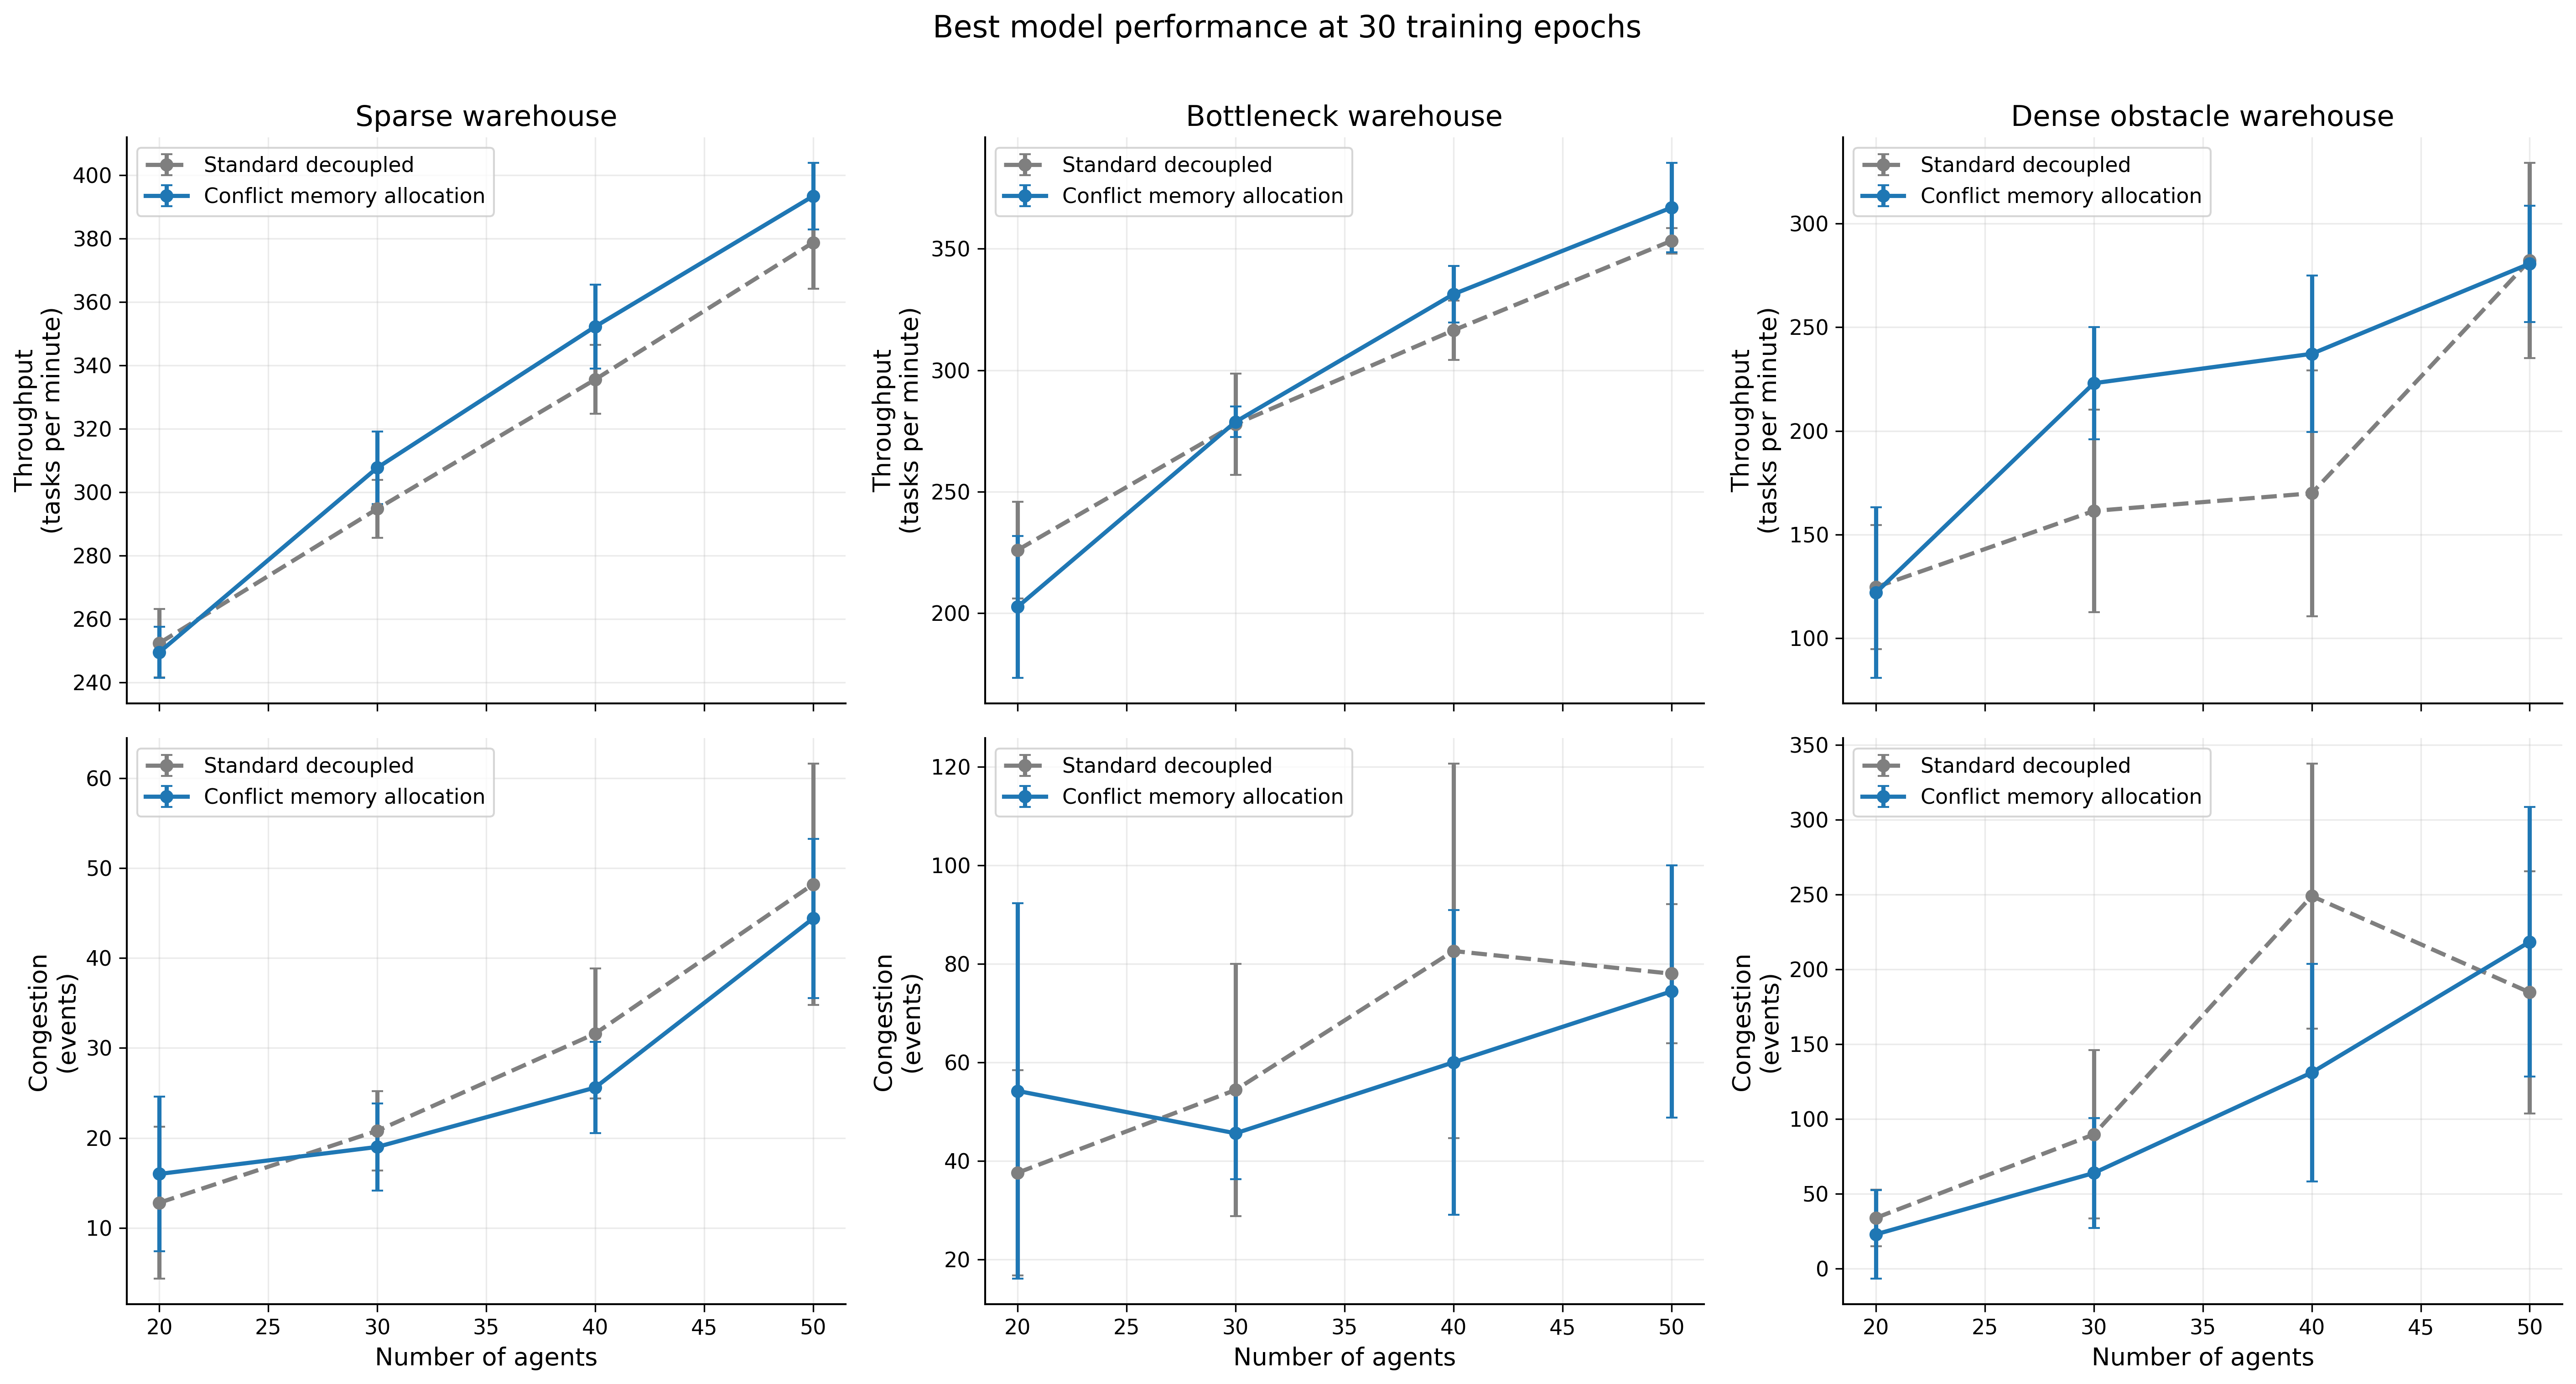
\includegraphics[width=\textwidth]{figure_4_throughput_and_congestion_comparison.png}
\caption{Best-model comparison at 30 training epochs. Top row: throughput. Bottom row: occupancy-based congestion events. Error bars summarize run-to-run variation across the 5 evaluation episodes. CMA improves throughput most clearly in dense-obstacle layouts at 30--40 agents and in bottleneck layouts at 40--50 agents. Low-load settings are often worse, and the 50-agent behavior is usually smaller or less consistent than the medium-load gains.}
\label{fig:main}
\end{figure}

\paragraph{The method is highly environment dependent.}
Averaging over agent counts makes the instability even clearer. In the sparse warehouse, mean throughput improvement across 30/60/90/120 epochs is approximately $3.0$, $-1.3$, $1.3$, and $-0.3$\%. In the bottleneck warehouse it is about $-0.3$, $3.1$, $6.8$, and $5.5$\%. In the dense-obstacle warehouse it is about $18.8$, $2.8$, $-6.7$, and $2.5$\%. Congestion prevention is similarly erratic: sparse is near zero or negative after 30 epochs, bottleneck improves steadily from about $1$\% to $26.8$\%, and dense swings from about $22.5$\% at 30 epochs to roughly $-27.5$\% at 90 epochs before recovering. The corresponding plots are given in \Cref{fig:training_improvement_app,fig:training_prevention_app}.

These trends show that CMA is most promising where topology creates repeatable bottlenecks, but the useful signal is narrow. In easier layouts, the added cost term can simply inject noise. In harder layouts, overtraining can also hurt, presumably because the predictor becomes better at the surrogate target without becoming better calibrated for assignment-time decisions.

\paragraph{Takeaway.}
The core hypothesis---that structured congestion information is reusable---receives partial support. The dense-obstacle and bottleneck results would be hard to explain if the memory map contained no signal at all. But the stronger claim---that a lightweight learned memory reliably fixes decoupled scheduling---is not supported by this prototype. The current proxy is too weak, and its training objective is too detached from the downstream decision.

\section{Conclusion}
\label{sec:conclusion}

We tested a lightweight feedback loop for decoupled multi-agent scheduling in which a learned congestion map modifies assignment costs. The result is encouraging but not decisive. CMA can improve throughput and reduce congestion in structured, congested layouts, and the gains at medium load can be substantial. At the same time, performance is brittle across training length, environment, and agent count, and the best predictive model is not the best scheduler.

For this workshop, that mismatch is the main message. ``Conflict memory'' is a plausible direction, but proxy congestion prediction is not yet a dependable substitute for real path-planning conflict information. The most important next step is to replace the occupancy surrogate with actual MAPF conflict logs and to tune the memory representation using downstream scheduling utility rather than prediction loss alone.

\bibliography{references}
\bibliographystyle{iclr2025}

\appendix

\section*{\LARGE Supplementary Material}

\section{Implementation and Selection Details}
The predictor uses three convolutional layers with hidden width 64 and ReLU activations. Inputs are two $20 \times 20$ channels, one for agent occupancy and one for active-task occupancy, and the network outputs a single $20 \times 20$ congestion map. The training target uses a lookahead horizon of 5 steps with inverse-step discounting.

CMA uses the same greedy matcher as the standard decoupled baseline and differs only through the additional path penalty in \cref{eq:cma-cost}. The fixed penalty weight is $\lambda=0.5$. Checkpoints are evaluated at 30, 60, 90, and 120 epochs. The selected checkpoint is the one with the largest mean throughput improvement aggregated across all 12 layout/load configurations, which is why the final choice differs from validation-loss selection.

\section{Additional Sensitivity Plots}

\begin{figure}[h]
\centering
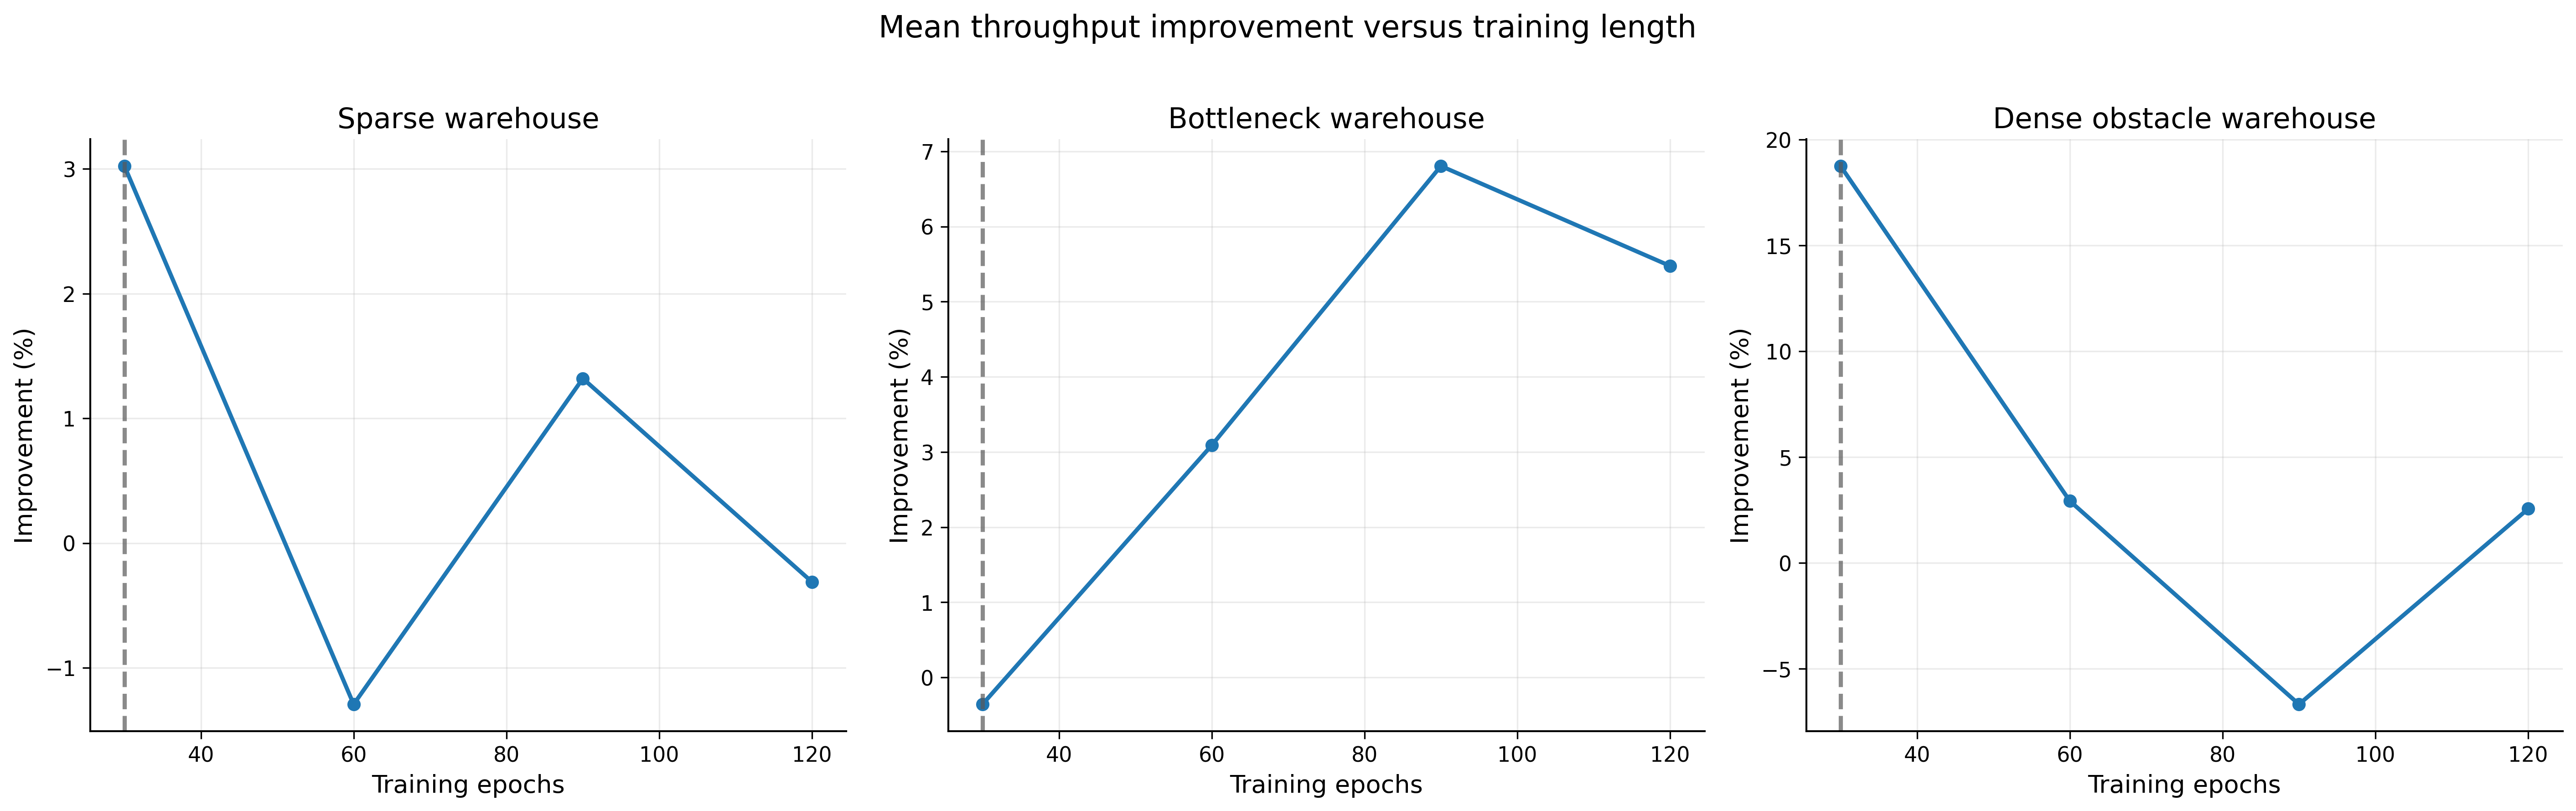
\includegraphics[width=\textwidth]{figure_6_training_length_improvement.png}
\caption{Mean throughput improvement versus training length, averaged over agent counts within each layout. Values are percentages relative to the standard decoupled baseline. The dashed vertical line marks the selected 30-epoch checkpoint. Early checkpoints are best in the dense-obstacle layout, while bottleneck performance improves later, illustrating that training length effects are environment dependent and non-monotonic.}
\label{fig:training_improvement_app}
\end{figure}

\begin{figure}[h]
\centering
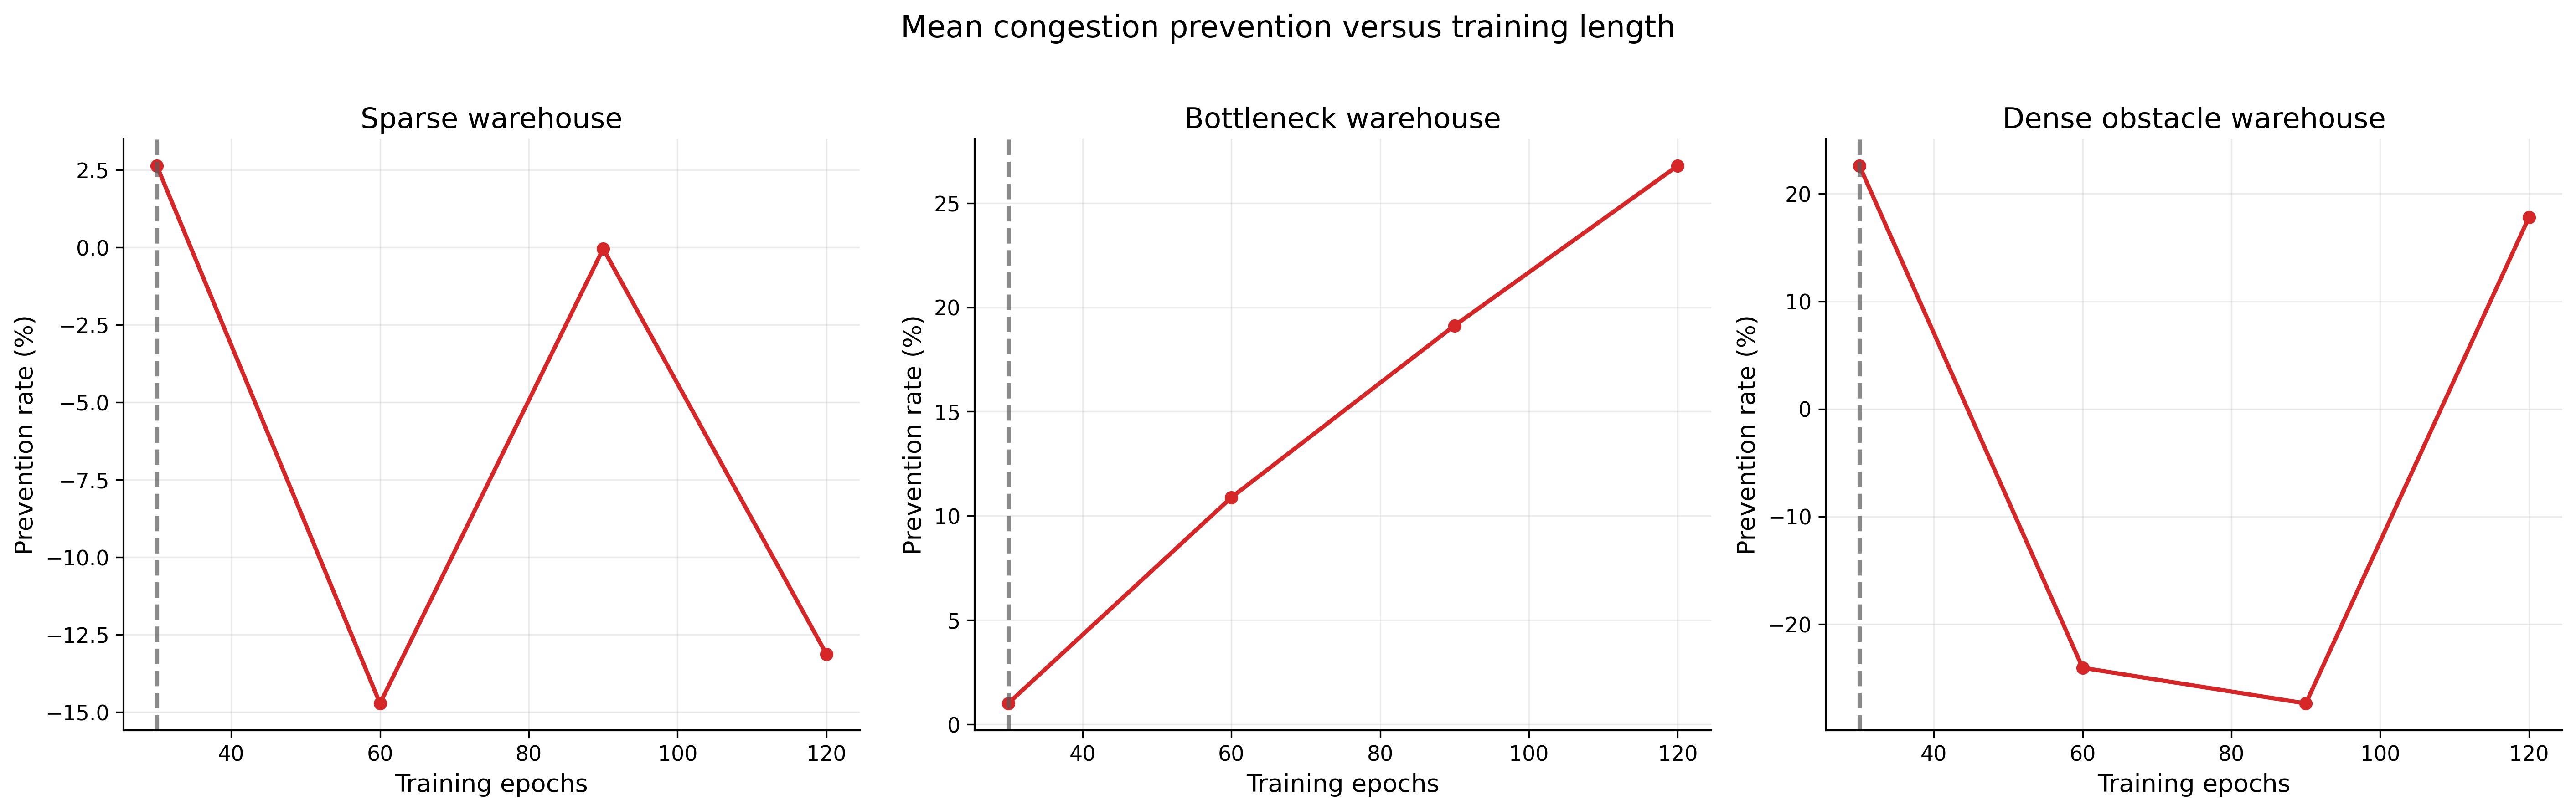
\includegraphics[width=\textwidth]{figure_7_training_length_prevention.png}
\caption{Mean congestion prevention versus training length, averaged over agent counts within each layout. Here prevention means percentage reduction in occupancy-based congestion relative to the standard decoupled baseline; negative values mean CMA produces more congestion. The dashed vertical line marks the selected 30-epoch checkpoint.}
\label{fig:training_prevention_app}
\end{figure}

\begin{figure}[h]
\centering
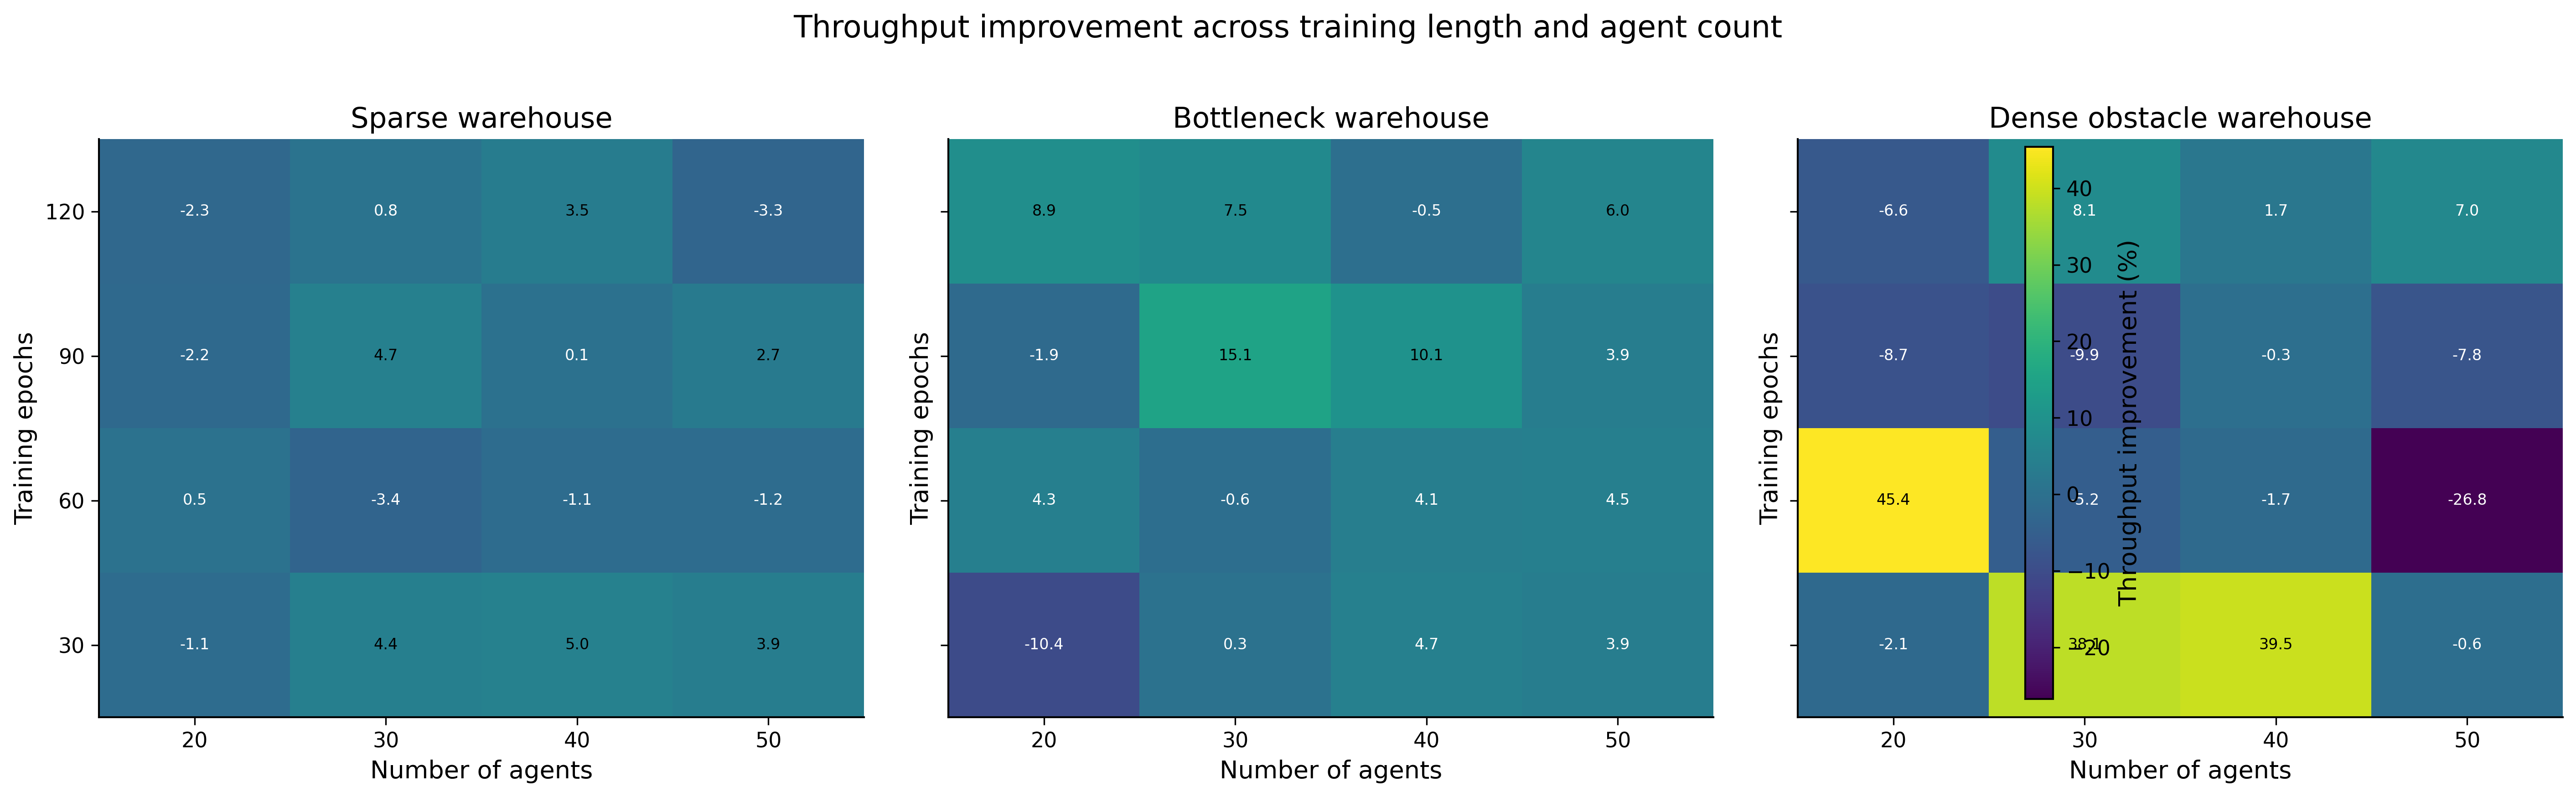
\includegraphics[width=\textwidth]{figure_2_improvement_heatmaps.png}
\caption{Throughput improvement across training length and agent count. Each cell is the percentage throughput change of CMA relative to the standard decoupled baseline for one layout, checkpoint, and agent count. Sparse layouts stay close to zero, bottleneck layouts show moderate positive regions, and dense-obstacle layouts have the largest upside as well as the largest failures.}
\label{fig:heat_improvement_app}
\end{figure}

\begin{figure}[h]
\centering
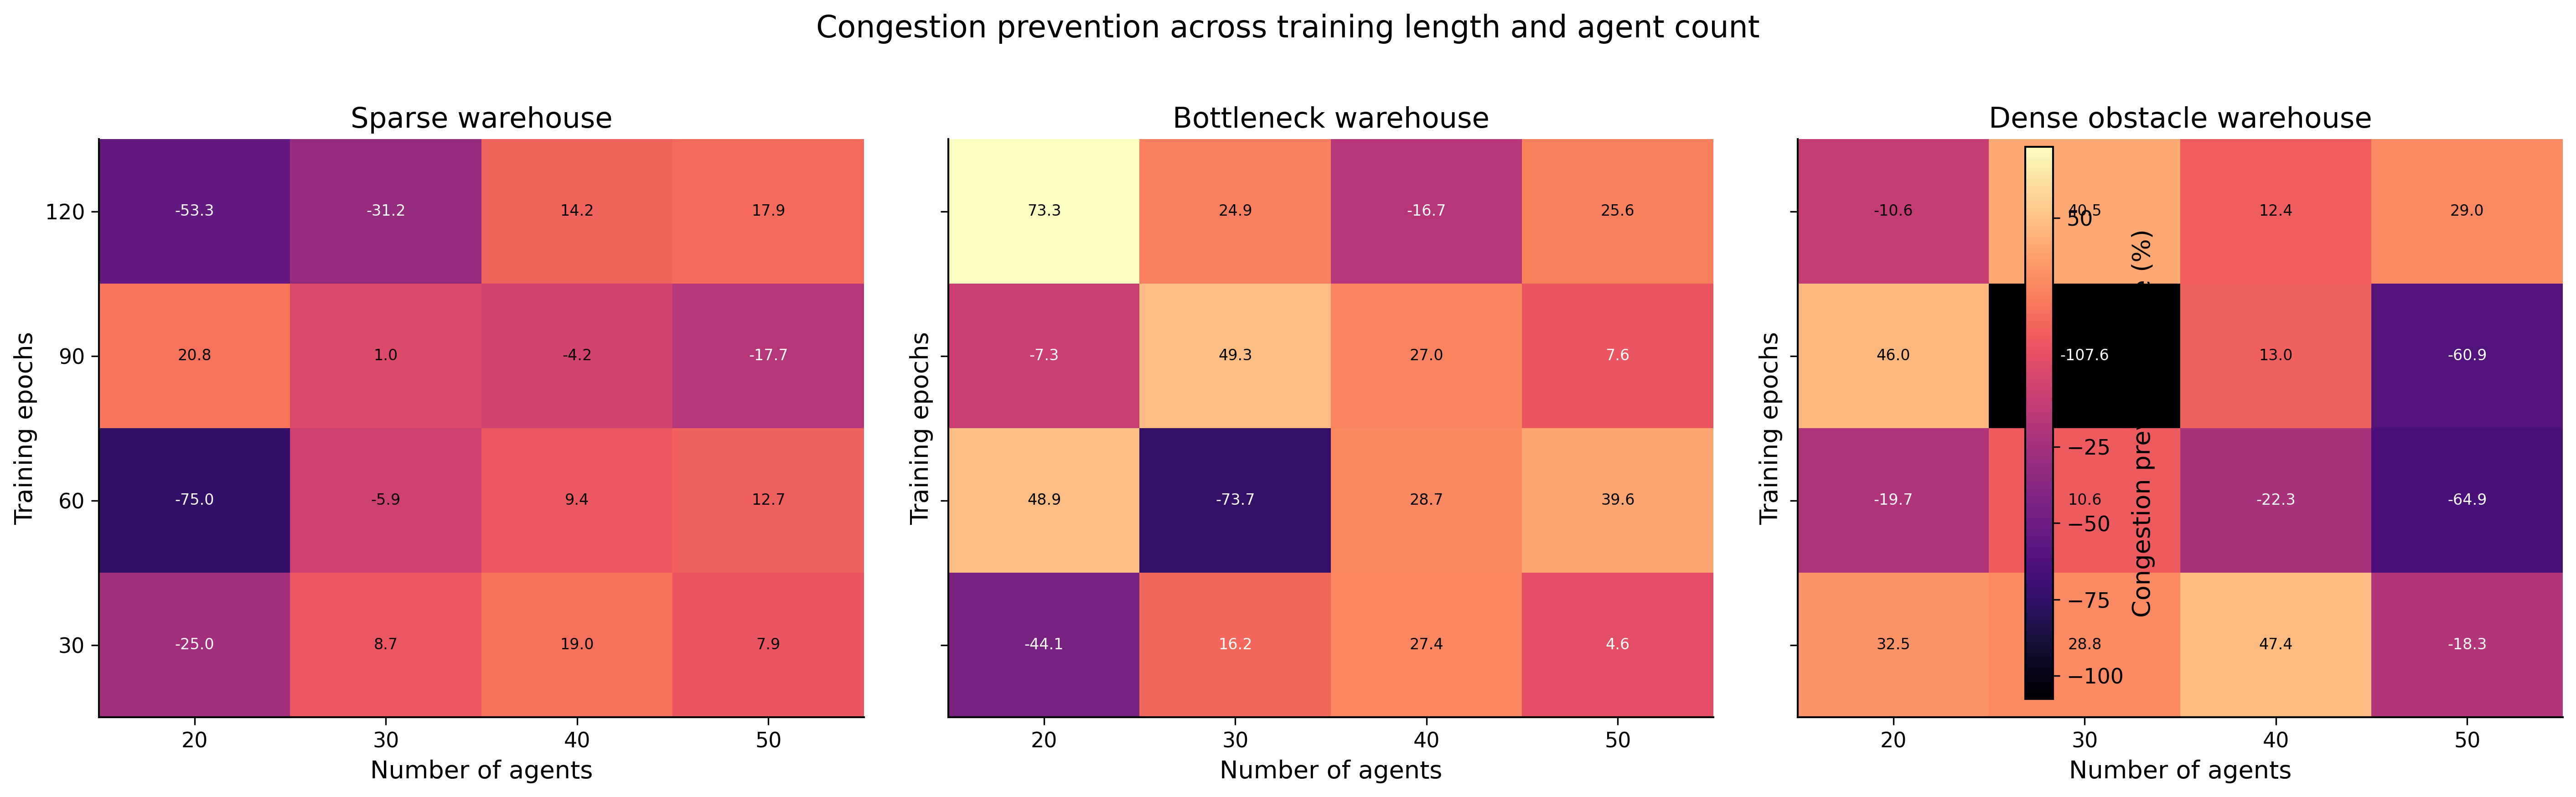
\includegraphics[width=\textwidth]{figure_3_congestion_prevention_heatmaps.png}
\caption{Congestion prevention across training length and agent count. Each cell is the percentage reduction in occupancy-based congestion relative to the standard decoupled baseline; negative values indicate worse congestion under CMA. The metric is highly checkpoint sensitive in the bottleneck and dense-obstacle layouts.}
\label{fig:heat_prevention_app}
\end{figure}

\begin{figure}[h]
\centering
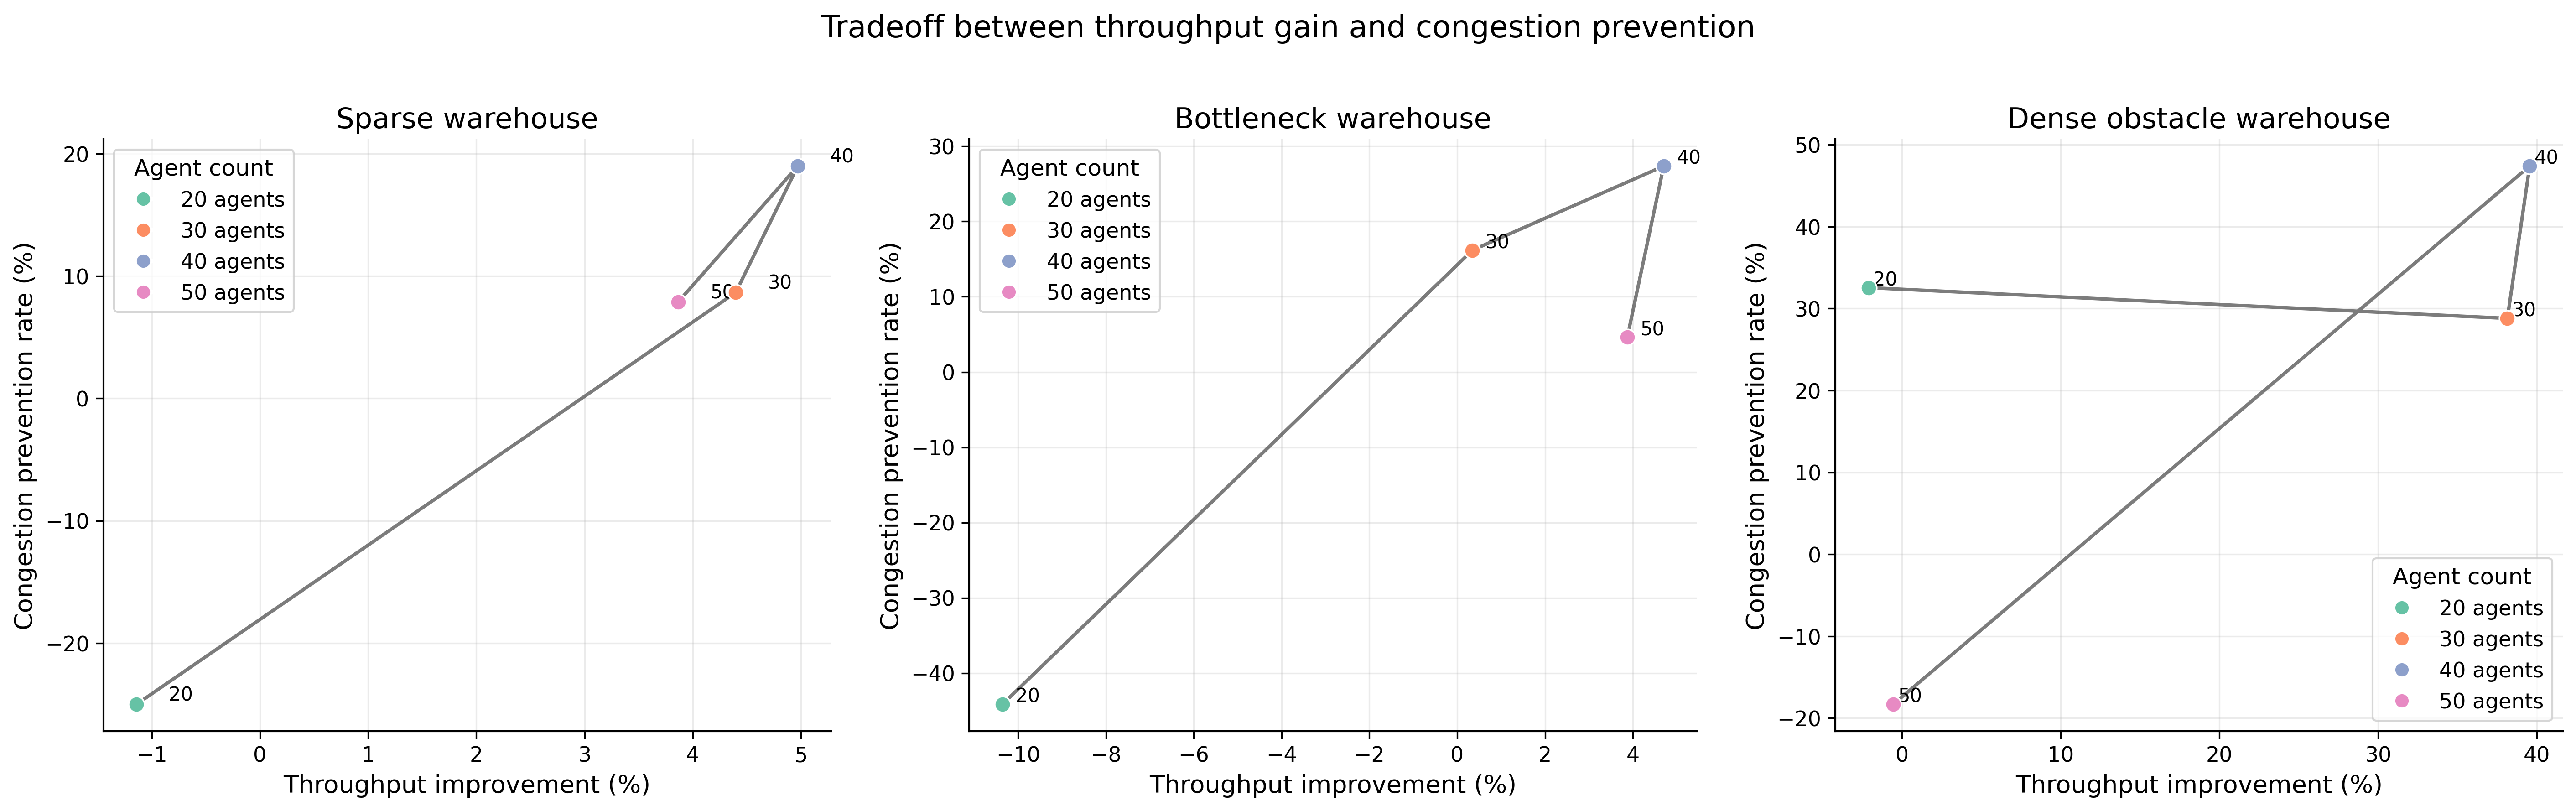
\includegraphics[width=\textwidth]{figure_8_tradeoff_analysis.png}
\caption{Tradeoff between throughput gain and congestion prevention at the selected 30-epoch checkpoint. Each point is one agent count in one layout, and points are connected only to show progression from 20 to 50 agents. Medium-load settings, especially in bottleneck and dense-obstacle layouts, usually offer the best joint tradeoff, but the relation between the two metrics is not strictly monotone.}
\label{fig:tradeoff_app}
\end{figure}

\end{document}